\chapter{System Design}
\label{chap:system_design}

This chapter outlines the architectural blueprint of \textbf{BookSphere}. We begin by describing the high-level system design and technology stack, followed by a detailed analysis of functional and non-functional requirements, and concluding with the visual interface design.

\section{System Architecture}
The BookSphere platform is built upon a robust \textbf{3-Tier Architecture}, designed to ensure separation of concerns, scalability, and maintainability.

\subsection{Architectural Layers}
\begin{itemize}
    \item \textbf{Presentation Layer (Frontend):} The client-side application is designed to be responsive and intuitive. It communicates with the backend via RESTful APIs, handling user interactions and data visualization (e.g., rendering the social graph or library shelves).
    
    \item \textbf{Logic Layer (Backend):} The core of the system is developed using \textbf{Java} with the \textbf{Spring Boot} framework. This layer handles business logic, security (Authentication/Authorization), and acts as an orchestrator between the two different databases. We utilize \textbf{Lombok} to reduce boilerplate code and ensure cleaner class definitions.
    
    \item \textbf{Data Layer (Polyglot Persistence):} The system adopts a hybrid storage strategy:
    \begin{itemize}
        \item \textbf{MongoDB:} Acts as the primary document store for Books, User Profiles, and detailed Reviews.
        \item \textbf{Neo4j:} Serves as the high-performance graph engine to manage social connections (\textit{FOLLOWS}) and interaction patterns (\textit{READS}, \textit{LIKED}) for the recommendation algorithms.
    \end{itemize}
\end{itemize}


\section{Requirements Analysis}
\subsection{Main Actors}
The system serves three main categories of users, each with distinct privileges and interaction capabilities:

\begin{itemize}
    \item \textbf{Administrator:} The super-user responsible for platform management. Their tasks range from maintaining the consistency of the catalog (adding/updating books and authors) to community moderation (deleting content and banning users).
    \item \textbf{Registered User:} The primary target audience of the platform. These users can fully interact with the system by creating social connections, writing reviews, curating their library, and generating personal analytics.
    \item \textbf{Unregistered User (Guest):} Users who access the platform in \textit{"read-only"} mode. They can explore the catalog, view public rankings and reviews, but cannot perform active interactions (rating, following, posting).
\end{itemize}

\subsection{Functional Requirements}
The functional requirements define the specific behaviors and functions of the system, categorized by the actor scope.

\subsubsection{General \& System Requirements}
These requirements apply to the core logic of the platform and are available to all users (including Guests) or performed automatically by the system background processes.

\paragraph{Search \& Discovery}
\begin{enumerate}
    \item The System must permit users to search for books and authors using different filters (genre, year, name).
    \item The System must allow users to search for other profiles and view their reviews.
    \item The System must enable any user to read reviews associated with a book.
\end{enumerate}

\paragraph{System Analytics \& Computation}
\begin{enumerate}
    \setcounter{enumi}{3} % Continua numerazione
    \item The System must compute, for every newly added book, a probability score indicating the likelihood of the book going viral.
    \item The System must compute a metric representing an author's versatility based on the variety of genres covered in their works.
    \item The System must compute a "How Far a Book Travels" index, measuring the geospatial distribution of a book's readers across the globe.
    \item The System must generate various rankings, such as top books or authors, filtered by year or genre.
    \item The System must calculate and display the average rating for authors and books for every year.
    \item The System must identify trending books based on the volume of reviews and ratings in the current month.
    \item The System must automatically identify "Influencers" within the application based on engagement quality metrics.
\end{enumerate}

\paragraph{Access}
\begin{enumerate}
    \setcounter{enumi}{10} % Continua numerazione
    \item The System must enable an Unregistered User to create a new account (Sign-up).
\end{enumerate}

\subsubsection{Registered User Requirements}
These features are exclusive to authenticated users.

\paragraph{Personalization \& Insights}
\begin{enumerate}
    \item The System must provide book recommendations based on the user's interaction history (favorite genres, authors) and global trends.
    \item The System must generate a "Wrapped" style summary of the user's reading year (statistics, top genres).
    \item The System must enable users to view a complete list of publications for a specific author.
    \item The System must allow users to retrieve all reviews for a specific book on demand.
\end{enumerate}

\paragraph{Content Creation \& Library Management}
\begin{enumerate}
    \setcounter{enumi}{4} 
    \item The System must allow a user to review books, providing a numerical evaluation (score) and an optional written comment.
    \item The System must allow each user to assign a status to a book, selecting from: \textit{To-Read}, \textit{Reading}, or \textit{Read}.
    \item The System must enable users to create and manage custom lists of books.
\end{enumerate}

\paragraph{Social Interaction}
\begin{enumerate}
    \setcounter{enumi}{7} 
    \item The System must enable users to follow other profiles and view their latest activities in a dedicated feed.
    \item The System must enable users to "like" or "unlike" specific books.
    \item The System must enable users to "like" or "unlike" reviews written by others.
    \item The System must allow users to view their list of friends/followed accounts.
\end{enumerate}

\paragraph{Account Management}
\begin{enumerate}
    \setcounter{enumi}{11} 
    \item The System must permit users to Log In and Log Out securely.
    \item The System must allow users to delete their account.
\end{enumerate}

\subsubsection{Administrator Requirements}
Privileged operations for content and user management.

\paragraph{Catalog Management}
\begin{enumerate}
    \item The System must enable an Admin to add new books, authors, or genres to the database.
    \item The System must enable an Admin to update existing information related to books, authors, or genres.
    \item The System must enable an Admin to remove a specific book, author, or genre.
\end{enumerate}

\paragraph{Moderation \& Oversight}
\begin{enumerate}
    \setcounter{enumi}{3}
    \item The System must allow an Admin to view the profile and data of any Registered User.
    \item The System must enable an Admin to view any review posted on the platform.
    \item The System must enable an Admin to delete reviews deemed inappropriate.
    \item The System must enable an Admin to ban a Registered User\footnote{Banning prohibits access but preserves specific user metadata to prevent re-registration with the same credentials.}.
\end{enumerate}

\subsection{Non-Functional Requirements}
These requirements define the quality attributes of the system.

\begin{enumerate}
    \item The System must follow RESTful design principles for API communication.
    \item The System must implement backup and redundancy strategies to avoid permanent data loss.
    \item The System must encrypt sensitive user data, specifically passwords, using industry-standard hashing algorithms.
    \item The System must be highly available and fault-tolerant to ensure continuous service.
    \item The System must enforce an Eventual Consistency model between the Document Database (MongoDB) and the Graph Database (Neo4j) to optimize performance over strict synchronization.
\end{enumerate}

\section{Expected Workload Distribution}
\label{sec:workload_distribution}

A critical aspect considered when designing the system and database architecture is the expected workload profile. Given the social nature of the application, BookSphere is designed to handle a \textbf{Read-Heavy} workload, typical of large-scale social platforms.

\subsection{Workload Profile (OLTP vs. OLAP)}
The system operates primarily as an \textbf{OLTP (Online Transaction Processing)} environment, characterized by a high volume of short, atomic transactions (e.g., posting a review, following a user). However, features such as \textit{Yearly Wrapped} and \textit{Trending Probability} introduce periodic \textbf{OLAP (Online Analytical Processing)} workloads, requiring the aggregation of vast datasets.

The operational split is estimated as follows:

\begin{itemize}
    \item \textbf{Read Operations ($\sim$80-85\%):}
    The majority of traffic consists of content consumption: browsing book details, traversing the social graph (viewing friends' activities), and authentication.
    \begin{itemize}
        \item \textit{Architectural Implication:} This imbalance justifies the use of \textbf{Replica Sets} in MongoDB. By setting the read preference to \texttt{secondaryPreferred}, we offload the heavy read traffic to secondary nodes, keeping the Primary free for write operations.
    \end{itemize}

    \item \textbf{Write Operations ($\sim$15-20\%):}
    Writes are further categorized based on frequency and complexity:
    \begin{enumerate}
        \item \textbf{High-Frequency Writes ($\sim$10-15\%):} Lightweight interactions such as 'Likes' and 'Follows'. These require low latency and can tolerate \textit{Eventual Consistency}.
        \item \textbf{Low-Frequency Writes ($<$5\%):} Content creation tasks such as writing detailed Reviews, rating books, and Administrative operations (CRUD on the catalog). These may require stricter validation.
    \end{enumerate}
\end{itemize}

\section{UML Class Diagram}
\label{sec:uml_diagram}

To provide a comprehensive view of the system's static structure and the relationships between entities, we present the UML Class Diagram in Figure \ref{fig:uml}. 




\begin{figure}[h]
    \centering
    % Assicurati che il file si chiami 'uml_diagram.svg' e sia nella stessa cartella
    % Non serve scrivere l'estensione .svg nel comando
    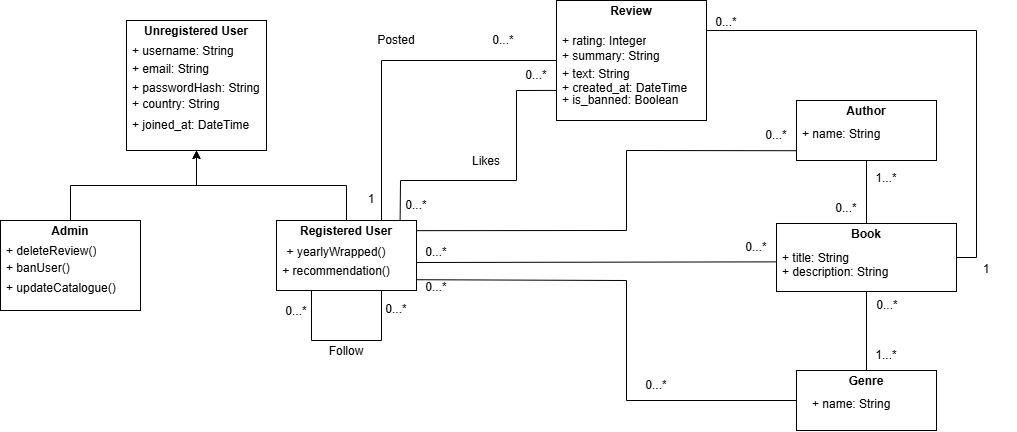
\includegraphics[width=1\textwidth]{img/UML.png}
    \caption{UML Class Diagram of BookSphere.}
    \label{fig:uml}
\end{figure}



% =============================================================================
% SECTION: UI MOCK-UPS
% =============================================================================

\section{User Interface Concept and Mock-ups}

This section presents the mock-ups developed to provide a conceptual visualization of the system’s user interface. These designs serve as a bridge between the functional requirements analyzed in the previous section and the final API implementation.

\begin{quote}
    \textit{\textbf{Note:} These mock-ups are intended for informational purposes only and were not implemented in the final system due to the project’s focus on API-based architecture. However, they demonstrate how the defined requirements would translate into a frontend user experience.}
\end{quote}

The following figures illustrate the interface design for the three main system actors: **Unregistered Users**, **Registered Users**, and **Administrators**.

% -----------------------------------------------------------------------------
% SUBSECTION: UNREGISTERED USER (GUEST)
% -----------------------------------------------------------------------------

\subsection{Unregistered User Experience}
The Guest interface focuses on \textbf{Search \& Discovery} and \textbf{System Analytics}, allowing users to explore the catalog without barriers before converting via the \textbf{Access} requirements.

\begin{figure}[H]
    \centering
    \begin{subfigure}[b]{0.45\textwidth}
        \centering
        % PLACEHOLDER FOR CLAUDE
        \fbox{\begin{minipage}{\textwidth}
            \centering
            \vspace{2cm}
            \textbf{[Landing Page with Search Bar]}
            \vspace{2cm}
        \end{minipage}}
        \caption{Landing Page \& Discovery \\ \textit{Satisfies General Req 1 (Search) \& Req 11 (Sign-up)}}
        \label{fig:mockup_guest_search}
    \end{subfigure}
    \hfill
    \begin{subfigure}[b]{0.45\textwidth}
        \centering
        % PLACEHOLDER FOR CLAUDE
        \fbox{\begin{minipage}{\textwidth}
            \centering
            \vspace{2cm}
            \textbf{[Book Detail View with Metrics]}
            \vspace{2cm}
        \end{minipage}}
        \caption{Public Analytics View \\ \textit{Satisfies General Req 4 (Viral Score) \& Req 9 (Yearly Ratings)}}
        \label{fig:mockup_guest_stats}
    \end{subfigure}
    \caption{Guest interface focusing on discovery and public data visualization.}
    \label{fig:mockup_guest_group}
\end{figure}

% -----------------------------------------------------------------------------
% SUBSECTION: REGISTERED USER
% -----------------------------------------------------------------------------

\subsection{Registered User Experience}
The Authenticated User interface enables **Personalization**, **Content Creation**, and **Social Interaction**. The designs below highlight the transition from passive reading to active engagement.

% FIGURE: FEED AND ACTIONS
\begin{figure}[H]
    \centering
    \begin{subfigure}[b]{0.45\textwidth}
        \centering
        % PLACEHOLDER FOR CLAUDE
        \fbox{\begin{minipage}{\textwidth}
            \centering
            \vspace{2cm}
            \textbf{[User Home Feed]}
            \vspace{2cm}
        \end{minipage}}
        \caption{Social Feed \& Recommendations \\ \textit{Satisfies Reg-Req 1 (Recs) \& Req 8 (Follow Feed)}}
        \label{fig:mockup_reg_feed}
    \end{subfigure}
    \hfill
    \begin{subfigure}[b]{0.45\textwidth}
        \centering
        % PLACEHOLDER FOR CLAUDE
        \fbox{\begin{minipage}{\textwidth}
            \centering
            \vspace{2cm}
            \textbf{[Book Interaction Modal]}
            \vspace{2cm}
        \end{minipage}}
        \caption{Review \& Status Management \\ \textit{Satisfies Reg-Req 5 (Review/Score) \& Req 6 (Status: To-Read/Read)}}
        \label{fig:mockup_reg_action}
    \end{subfigure}
    \caption{Core interaction screens for Registered Users.}
    \label{fig:mockup_reg_core}
\end{figure}

% FIGURE: WRAPPED / INSIGHTS
\begin{figure}[H]
    \centering
    % Example of a single larger image for the "Wrapped" concept
    \fbox{\begin{minipage}{0.8\textwidth}
        \centering
        \vspace{2.5cm}
        \textbf{[User Year-in-Review "Wrapped" Design]}
        \vspace{2.5cm}
    \end{minipage}}
    \caption{Personalized Analytics Dashboard. \\ \textit{Satisfies Reg-Req 2 ("Wrapped" Summary)}}
    \label{fig:mockup_wrapped}
\end{figure}

% -----------------------------------------------------------------------------
% SUBSECTION: ADMINISTRATOR
% -----------------------------------------------------------------------------

\subsection{Administrator Experience}
The Admin interface prioritizes **Catalog Management** and **Moderation**. These views are data-dense to facilitate efficient system oversight.

\begin{figure}[H]
    \centering
    \begin{subfigure}[b]{0.45\textwidth}
        \centering
        % PLACEHOLDER FOR CLAUDE
        \fbox{\begin{minipage}{\textwidth}
            \centering
            \vspace{2cm}
            \textbf{[Catalog Management Table]}
            \vspace{2cm}
        \end{minipage}}
        \caption{Database Management \\ \textit{Satisfies Admin Req 1-3 (Add/Update/Remove)}}
        \label{fig:mockup_admin_catalog}
    \end{subfigure}
    \hfill
    \begin{subfigure}[b]{0.45\textwidth}
        \centering
        % PLACEHOLDER FOR CLAUDE
        \fbox{\begin{minipage}{\textwidth}
            \centering
            \vspace{2cm}
            \textbf{[User Moderation Panel]}
            \vspace{2cm}
        \end{minipage}}
        \caption{Moderation \& Banning \\ \textit{Satisfies Admin Req 7 (Ban User) \& Req 6 (Delete Review)}}
        \label{fig:mockup_admin_mod}
    \end{subfigure}
    \caption{Administrative panels for maintaining system integrity.}
    \label{fig:mockup_admin_group}
\end{figure}